\chapter{État de l’art}

  La problématique du passage à l’échelle des noyaux n’est pas nouvelle. Dès les
  années 90, ~\citeauthor{unrau1995hierarchical} posent la question et apportent
  des réponses avec le noyau Hurricane (détaillé en section
  \ref{subsec:others}). D’autres essaye avec le modèle des
  micro-noyaux, comme Minix~\citep{}, L4~\citep{} ou Mach~\citep{}. Mais c'est
  finalement Linux qui s’impose comme le modèle de référence, et les travaux se
  focalise alors sur ce dernier.

  Mais, aux alentours des années 2004/2005, un changement radical a été opéré de
  la part des constructeurs tels qu’Intel ou AMD. Plutôt que de continuer à
  augmenter la fréquence des processeurs, ce qui devenait contre productif vu la
  quantité d’énergie nécessaire, ils ont préféré augmenter le nombre de coeurs
  et le nombre de processeurs sur les puces. C'est le début du parallélisme
  massif~\citep{patterson2011parallel}, et c'est à ce moment là que la question
  du passage à l’échelle du noyau Linux fût soulevée.\\

  Cet état de l'art se concentre sur cette problématique, mais aborde également
  une autre thématique.En effet, l'architecture TSAR (voir~\ref{sec:tsar})
  implique de gérer un espace d'adressage physique considérablement plus grand
  que l'espace virtuel (4Go), à cause du choix des processeurs 32 bits. Cette
  situation, inédite, apporte le challenge de la gestion de ces espaces par le
  noyau. Nous verrons donc quelles solutions, matérielles comme logicielles,
  existent pour nous permettre de réaliser cela. Enfin, le passage d’ALMOS au
  mode multi-noyau nous permettra de nous intéresser aux problèmes soulevés par
  le maintient de la cohérence des données systèmes sur une machine lorsque l'on
  a plusieurs noyaux en cours d'exécution, ces derniers devant partager un
  minimum de ressources vitales à leur bon fonctionnement.

  \section{Passage à l’échelle des noyaux}
  \label{sec:scalability}

    \subsection{Scalabilité du noyau Linux}

      Il apparaît évident dans un premier temps de vouloir adapter le noyau
      Linux à des architectures massivement multi-c\oe urs. En effet, changer de
      noyau, alors que ce dernier s’est imposé partout, est un pari très risqué,
      et très difficile. À cet effet, ~\citet{boyd2010analysis} ont étudié la
      scalabilité de Linux sur une machine 48 c\oe urs en utilisant le benchmark
      MOSBENCH. Ils ont pu tirer plusieurs conclusions de cette étude.
      Premièrement, il existe trois types de problèmes liés au passage à
      l’échelle :
      \begin{itemize}
        \item l’implémentation du noyau
        \item l’implémentation de l’application utilisateur
        \item la faćon dont l’application utilise les services du noyau
      \end{itemize}
      Grâce à cela,~\citeauthor{boyd2010analysis} sont parvenus à résoudre les
      problèmes liés aux applications de MOSBENCH, et ce en utilisant des
      techniques basiques de programmation parallèle. De plus, la grande
      majorité de leurs contributions sur le noyau ne sont que de petits
      changements très localisés. À l’exception du mécanisme des \textit{sloppy
        counters} qu'ils ont introduit, aucun concept clé de Linux n'a été
      touché. \todo{Détailler les sloppy counters.}

      Ainsi, ils sont parvenus à identifier les problèmes du noyau, comme par
      exemple la gestion du cache des \texttt{dentry}, les goulots formés par
      les sytèmes de fichiers montés, etc\ldots, et à les résoudre pour obtenir
      des performances acceptables.

      Néanmoins, nous pouvons aujourd’hui adresser trois critiques à ces travaux
      :
      \begin{itemize}
        \item le noyau utilisé est ancien (2.6.35-rc5, 12 Juillet 2010). Les
          mécanismes de préemption venaient d’être ajoutés et n’étaient pas
          aussi performants qu'aujourd'hui
        \item la machine considérée est composée de seulement 48 coeurs, ce qui
          est peu par rapport à la puissance des machines actuelles
        \item leur propre conclusion indique qu’il ne faut pas changer le design
          des sytèmes d’exploitation `` pour l’instant''
      \end{itemize}
      Nous pensons qu’à présent, il est nécessaire de revoir cette organisation.

      
    \subsection{Popcorn Linux}

      Le projet Popcorn Linux~\citep{barbalacepopcorn} part du même constat
      évoqué précédement, mais en essayant tout de même de conserver le noyau
      Linux comme base de travail. Avec un noyau plus récent que l'étude
      précédente (3.2), ils ont en partie adopté les principes du multi-noyau
      mais en ont rejeté certains.\footnote{Notamment l'hétérogénéité des
        architectures~\citep{schupbach2008embracing} qui n'est pas du tout
        abordée dans ce projet.}\newline

      Popcorn Linux permet de lancer plusieurs noyaux Linux en même temps sur la
      même machine. Le matériel est attribué de manière logicielle entre les
      différentes instances du noyau, et ces dernières communiquent uniquement
      par passage de messages. Afin de garantir à l’utilisateur l’illusion d’un
      seul système en cours d'exécution, ils ont utilisé les mécanismes de
      \textit{namespace} offert par Linux pour construire ce qu’ils nomment ``
      l’image disque unique'' (\textit{Single System Image},
      figure~\ref{fig:popcorn-layers}). \todo{Expliquer les namespaces}

      \begin{figure}[h]
        \centering
        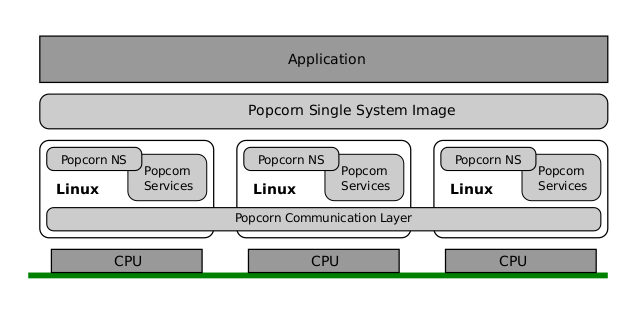
\includegraphics[scale=0.44]{popcorn-layers}
        \caption{Architecture logicielle du noyau Popcorn Linux. La couche de
          communication assure à l'utilisateur l'illusion d'un unique noyau.
          Source:~\citeauthor{barbalacepopcorn}}
        \label{fig:popcorn-layers}
      \end{figure}

      Le partitionnement des ressources est fait selon la configuration donnée
      au boot du noyau. Le premier noyau qui est lancé, appelé `` noyau
      maître'', lance un processus de reconnaissance du matériel. Ensuite, on
      précise aux noyaux secondaires, via des paramètres au boot les ressources
      dont ils peuvent disposer, en fonction de celles trouvées par le noyau
      maître. Une fois les noyaux lancés, ils ne partagent aucune données,
      exception faite de la table contenant les adresses d’écriture des buffers
      des autres noyaux, utilisée pour le passage de messages (voir
      figure~\ref{fig:popcorn-buf}). Ces buffers sont de types `` MWSR'', ou
      \textit{Multi Writer Single Reader}, et utilisent un système de ticket
      pour les écritures. Les lectures utilisent un mélange de deux
      techniques:\benumline \item le lecteur viendra consulter de manière
      régulière le contenu de son buffer (\textit{polling}) ou \item il ira lire
      le buffer sur réception d’une IPI (\textit{Inter-Processor Interruption})
      du coeur ayant initié l’écriture\eenumline.

      \begin{figure}[h]
        \centering
        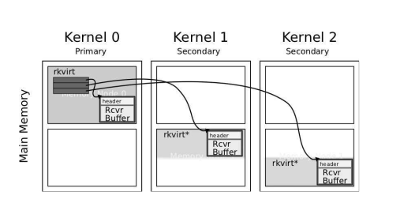
\includegraphics[scale=0.3]{popcorn-buffers}
        \caption{Les différents noyaux doivent impérativement mapper le tableau
          \texttt{rkvirt} dans leur espace d'adressage pour pouvoir communiquer
          avec les autres. L'adresse de ce tableau est fixe et connue de tous.
          Lorsqu'un noyau secondaire est lancé, il ajoute l'adresse de son
          buffer dans ce tableau. Source:~\citeauthor{barbalacepopcorn}}
        \label{fig:popcorn-buf}
      \end{figure}

      Ces communications permettent de donner l’illusion qu’il n’y a qu’un seul
      noyau en cours d’exécution, mais aussi de pouvoir migrer des tâches entre
      les différentes instances de noyaux de manière transparente.\newline

      Les tests de performances effectués sur Popcorn Linux se sont montrés
      décevants. D'une part parce que la machine considérée ne contient que 48
      coeurs et 64Go de mémoire, et d'autre part parce que les résultats des
      tests n'ont pas montrés d'améliorations significatives des
      performances. Au contraire, il apparaît que Popcorn Linux est
      majoritairement mois efficace que Linux, sauf dans quelques
      cas\footnote{L'utilisation de gmake pour la compilation noyau par
        exemple.}. Ce résultat est à relativiser, car une seul suite de
      benchmark a été utilisée ici. En revanche, ce projet ne s'attaque pas à la
      problématique des espaces d'adressages physiques très grands sur des
      architectures 32 bits.


    \subsection{Barrelfish}
      
      L’ETH Zurich, en collaboration avec Microsoft Research, a engagé des
      travaux de recherche dans le domaine des architectures du futur en
      2008. Leurs équipes sont parvenues à établir un nouveau modèle de
      construction des systèmes d’exploitation : le
      multi-noyau~\citep{schupbach2008embracing}. Ce paradigme part de plusieurs
      postulats\benumline \item les architectures du futur seront très
      hétérogènes \item les noyaux actuels ne profitent pas de l’hétérogénéité
      offerte par le matériel et au contraire essayent de la masquer un maximum
      \item les machines sont construites comme des systèmes distribués,
        pourquoi ne pas appliquer le même modèle aux systèmes
        d’exploitation~\citep{}\eenumline.\\

      \begin{figure}[h]
        \centering 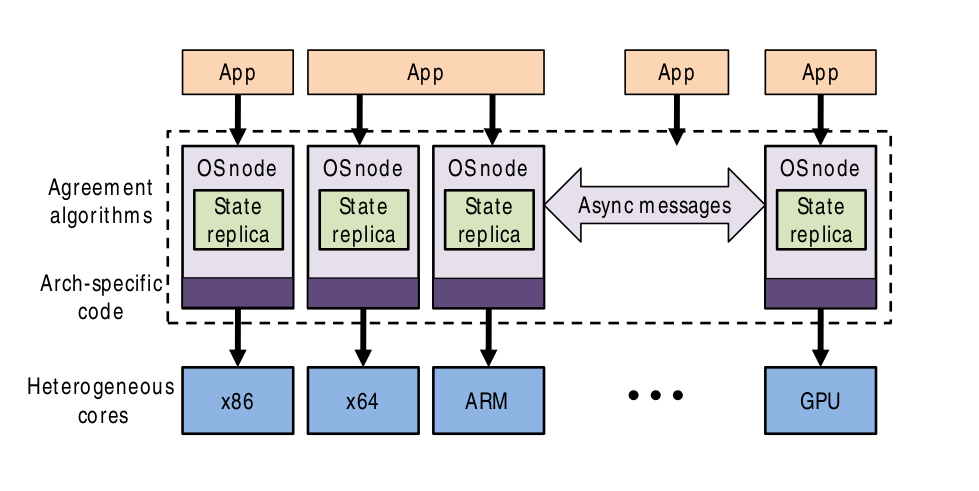
\includegraphics[scale=0.3]{barrelfish}
        \caption{L'architecture multi-noyau de Barrelfish. Source:
          \citeauthor{schupbach2008embracing}}
        \label{fig:barrelfish}
      \end{figure}
        
      Selon l’approche multi-noyau (voir figure~\ref{fig:barrelfish}),
      l'environnement d’exécution des applications est une collection de n\oe
      uds où chaque n\oe ud est constitué d’un c\oe ur exécutant un OS à base
      d’un micro-noyau. Les communications entre les différents OS se font par
      passage de messages : Barrelfish utilise une variante des Remote Procedure
      Calls au niveau utilisateur (URPC). chaque OS dispose d’un serveur système
      en mode utilisateur appelé Monitor. L’ensemble des moniteurs coordonne
      collectivement l’accès à l’état global du système et maintient la
      cohérence des structures de données répliquées par c\oe ur (les tables
      d’allocation mémoire et les mappings des espaces d’adressages
      virtuels).\newline

      \todo{Résultats de benchmark ici.}

    \subsection{Autres travaux}
    \label{subsec:others}
    
      \begin{paragraph}{Hurricane:}

        Parmi les premiers travaux sur la scalabilité des systèmes
        d’exploitation se trouve la thèse d’Unrau. Celui-ci a formulé trois
        grands principes pour une conception scalable d’un système
        d’exploitation qui sont : \benumline \item préserver le
        parallélisme \item borner le surcoût des services et \item préserver la
        localité\eenumline. \citet{unrau1995hierarchical} ont proposé le système
        d’exploitation Hurricane à base de micro-noyau avec une approche de
        conception nommée Hierarchical Clustering.\newline

        Selon cette approche, le système d’exploitation est vu en tant qu’une
        collection de clusters. Un cluster est un système d’exploitation complet
        à base de micro-noyau prenant en charge un faible nombre de
        processeurs. Il existe donc autant d’instances du système d’exploitation
        que de clusters. Les serveurs systèmes (en mode utilisateur) de chaque
        cluster coopèrent entre eux pour donner aux applications une vision
        globale d’un seul système d’exploitation. Étant donné que chaque cluster
        propose l’ensemble des services système via des serveurs dédiés,
        l’existence de plusieurs clusters constitue une réplication des mêmes
        services et augmente la disponibilité du système. La dimension (en
        nombre de processeurs) d’un cluster est un compromis entre le coût des
        accès intra-cluster et inter-clusters.\newline

        %% La figure~\ref{fig:hurricane} illustre l’organisation de plusieurs
        %% clusters pour constituer un système distribué fortement couplé.

        %% \begin{figure}[h]
        %%   \centering 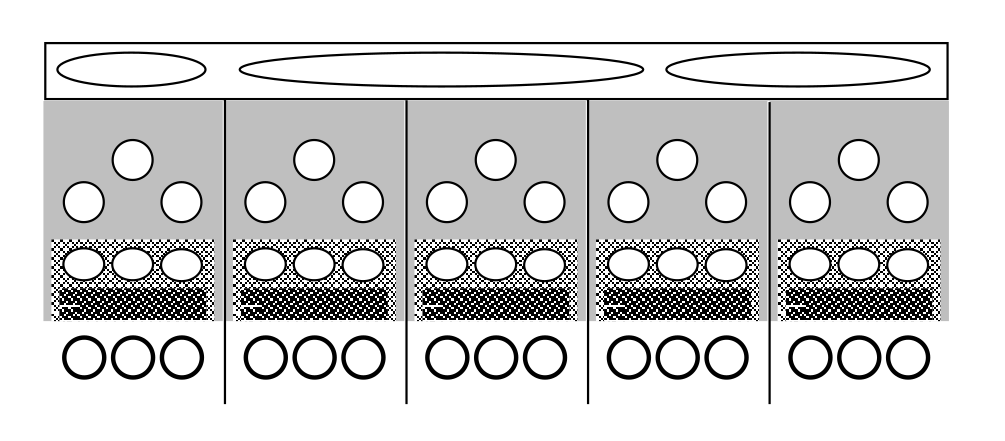
\includegraphics[scale=0.2]{hurricane}
        %%   \caption{Un système multi-cluster. Source:
        %%     \citet{unrau1995hierarchical}}
        %%   \label{fig:hurricane}
        %% \end{figure}

        Un envoi de message est réalisé par l’interruption du cluster cible
        pour\benumline \item l’allocation d’un tampon mémoire pour réceptionner
        le message \item copier le message et les informations de contrôle
        depuis le processus émetteur du cluster source et \item attacher le
        tampon à la file d’attente du processus destinataire du
        message\eenumline. Quand un client demande un service, il change son
        espace d’adressage pour celui du serveur et invoque un thread de
        traitement associé à sa requête avant de retrouver son espace
        d’adressage initial.

      \end{paragraph}
      
      \begin{paragraph}{Corey:}

        Avant leurs travaux sur Linux,~\citet{boyd2008corey}. ont proposé le
        système d’exploitation Corey. Dans ce dernier, la gestion du partage des
        ressources est laissée aux applications utilisateurs.

        En donnant le contrôle aux programmeurs des applications utilisateur,
        Corey permet en effet de personnaliser le comportement du noyau selon
        les besoins et les spécificités d’une application. Les inconvénients
        majeurs de cette approche sont: \benumline \item lier fortement
        l’application au système qui l’exécute, ce qui élimine complètement ou
        partiellement la portabilité des applications et complique sérieusement
        la réutilisation du code existant \item augmenter la complexité de
        programmation et nécessiter d’avantage d’efforts de la part des
        programmeurs d’applications (gestion explicite des régions virtuelles,
        placement et partage des structures de données noyau, etc.) et \item
        générer des conflits dans le cas d'exécutions simultanées des
        applications\eenumline.

      \end{paragraph}

      \begin{paragraph}{FoS:}

        Des travaux de recherches similaires visant à repenser le système
        d’exploitation sous forme d’une collection d’OS communicants par passage
        de messages ont été menés par~\citet{wentzlaff2009factored} avec
        FoS. L’objectif du projet FoS est de concevoir un système à la fois pour
        processeurs many-cores et pour les infrastructures de Cloud
        Computing. Comme dans le cas de Barrelfish, chaque c\oe ur exécute une
        instance de l’OS complet à base de micro-noyau comme il est illustré par
        la figure~\ref{fig:fos}.

        \begin{figure}[h]
          \centering
          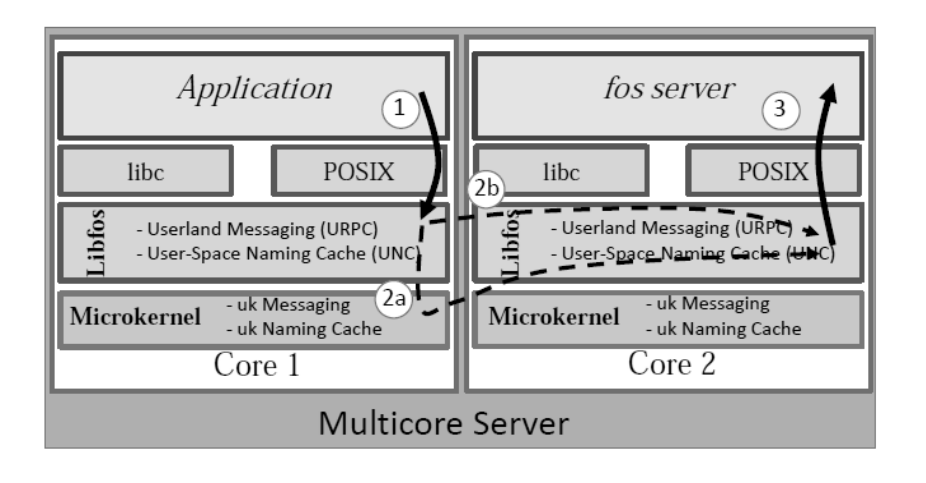
\includegraphics[scale=0.3]{fos}
          \caption{Apercu de la structure interne du noyau FoS et du schéma de
            communication}
          \label{fig:fos}
        \end{figure}

        \todo{Dire qu'on peut attribuer les ressources matérielles à certaines
          fonctionnalités.} En se fondant sur le partitionnement spatial des
        ressources de calcul, certaines instances de l’OS exécutent des serveurs
        systèmes, tandis que d’autres exécutent les applications. À la
        différence de Barrelfish, FoS se focalise sur la parallélisation des
        services systèmes pour faire face à une demande massive et variable de
        services.\\

        Concernant les évaluations expérimentales, les principales publications
        autour du projet FoS~\citep{wentzlaff2009factored,
          wentzlaff2010operating} n’incluent pas d'évaluations de scalabilité en
        utilisant des benchmarks.

      \end{paragraph}
      
    \subsection{Influences}

      Bien que ces travaux n'apportent pas de réponse claire et définitive à
      notre problématique, ils nous permettent de mieux comprendre les choix qui
      ont été fait dans le noyau ALMOS. Premièrement, les travaux sur Barrelfish
      ont apporté un nouveau modèle architectural pour la conception d'un
      noyau. Ce modèle semble cohérent et répond aux besoins des futures
      architectures. C'est donc le modèle qui a été retenu par
      ALMOS\footnote{Nous verrons plus en détail en section~\ref{sec:almos} le
        choix du multi-noyau.}. Néanmoins, Barrelfish ne respecte pas du tout
      les standards POSIX. C'est un choix très fort qui a été fait pour ce
      projet, et qui nous apparaît comme infondé.

      Les travaux sur Popcorn Linux, basé lui aussi sur le modèle du
      multi-noyau, ont permis de montrer que le noyau Linux, qui se veut être
      \textit{POSIX compliant}, peut être adapté à des architectures massivement
      parallèles, tout en respectant les normes. Le projet ALMOS, tout comme
      Popcorn Linux, a fait le choix d'avoir un système respectant au maximum
      les standards de conception des noyaux déja existants.

      Enfin, les notions de hiérarchisation et de clusters, initalement
      apportées par~\citet{unrau1995hierarchical} et poussées à l'extrême dans
      le noyau Barrelfish\footnote{Un cluster est composé d'un seul processeur
        et non pas un ensemble.}, sont maintenant parties intégrante de
      l'architecture TSAR et du noyau ALMOS.\\

      Pourtant, ces recherches ne répondent pas à un des problèmes majeurs de
      l'architecture TSAR. En partant du principe que les processeurs
      d'aujourd'hui manipulent des informations sur 64 bits, les problèmes de
      gestion d'une grande quantité de mémoire ont été effacés. Néanmoins, nous
      allons tout de même présenter en section~\ref{sec:memory} quelques
      solutions permettant de contourner ce problème, mais toujours de manière
      incomplète. Ces solutions seront une base de réflexion pour de futurs
      travaux au laboratoire.
    
     

  \section{Gestion des espaces d'adressage}
  \label{sec:memory}    

    \subsection{Physical Address Extension}

      Avant l'apparition des architectures 64 bits s'est posé la question de la
      gestion d'espaces d'adressage supérieurs à 4Go avec des processeurs 32
      bits. Les premiers travaux ont été menés par Intel et ont débouché sur la
      technologie PAE (\textit{Physical Address
        Extension})~\citep{patent6349380}. Celle-ci permet d'utiliser des
      adresses physiques sur 36 bits au lieu de 32, et donc d'exploiter jusqu'à
      64Go de mémoire.

      \begin{figure}[h]
        \centering 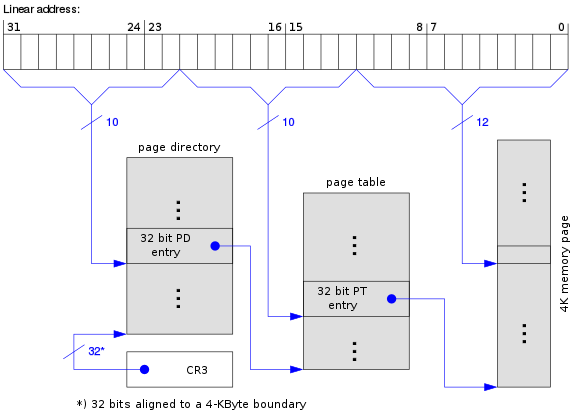
\includegraphics[scale=0.4]{paging-no-pae}
        \caption{Exemple de traduction d'adresse par la MMU sans utiliser la
          technologie PAE}
        \label{fig:paging-no-pae}
        \end{figure}
      
      Ce mécanisme fût introduit en 1995 dans les premiers Pentium Pro, et
      foncionne de la manière suivante. Considérons une MMU classique
      (figure~\ref{fig:paging-no-pae}) permettant de gérer des adresses de 32
      bits. Celle-ci contient deux niveaux d'indirection, chacun ayant 1024
      entrées de 4 octets. Lors d'une traduction, on utilise les MSB (Most
      Significant Bits) d'une adresse pour trouver les entrées correspondantes
      dans chacune des indirections, puis les LSB pour obtenir l'offset.

      Chaque processus à dans son espace virtuel un pointeur vers une adresse
      physique. À cette adresse se trouve le \textit{Page Directory}. Les
      entrées de ce tableau (appelées PDE pour \textit{Page Directory Entry})
      sont indexées par les 10 premiers bits de l'adresse virtuelle que l'on
      veut accéder. Elles sont stockées sur 32 bits, et le \textit{Page
        Directory} contient 1024 entrées ($2^{10} = 1024$). Les PDE contiennent
      le numéro de la page mémoire où est située la \textit{Page Table} du
      processus. Ce numéro est appelé PFN, pour \textit{Page Frame
        Number}. Comme le \textit{Page Directory}, la \textit{Page Table} est
      indexée par 10 bits. Elle a donc une profondeur de 1024, et les entrées
      (PTE) sont stockées sur 32 bits. Ces PTE contiennent le PFN de la page
      contennant la donnée que l'on cherche a accéder. À partir de ce PFN, on
      peut retrouver l'adresse physique de la page correspondante, puis on
      utilise les 12 bits d'offset restant pour se déplacer et obtenir la
      donnée.

      \begin{paragraph}{Remarque:}
        Le noyau Linux utilise quatre niveaux d'abstraction dans sa version
        actuelle. Néanmoins, ils sont purement logiciels. La MMU continue de
        travailler avec deux niveaux d'indirection comme dans la
        figure~\ref{fig:paging-no-pae}.\newline
      \end{paragraph}
      
      L'activation du mode PAE dans la MMU permet de rajouter un troisième
      niveau d'indirection, en diminuant le nombre de MSB utilisés
      précédement. On voit sur la figure~\ref{fig:paging-pae} que les bits 30 et
      31 sont maintenant réservés à une nouvelle table, la PDPT (\textit{Page
        Directory Pointer Table}). Le mode PAE transforme également la taille
      des entrées du \textit{Page Directory} et de la \textit{Page Table} en
      entrées de 64 bits et non plus 32. Pour ce faire, on diminue le nombre
      d'entrées possibles dans ces tables. En divisant par deux le nombre
      d'entrées possibles, soit 512 au lieu de 1024, au multiplie par deux la
      taille des données que l'ont peut stocker.

      \begin{figure}[h]
        \centering 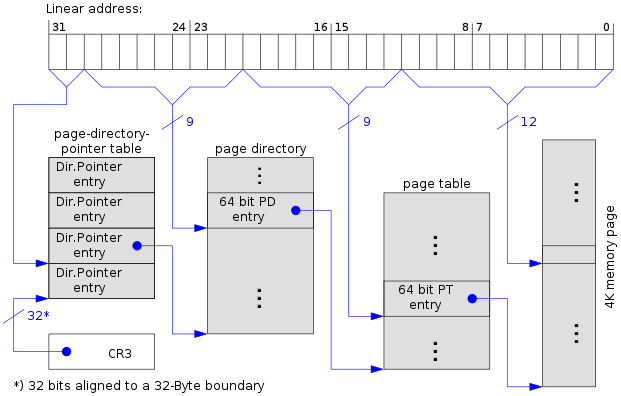
\includegraphics[scale=0.4]{paging-pae}
        \caption{Exemple de traduction d'adresse par la MMU avec la technologie
          PAE}
        \label{fig:paging-pae}
      \end{figure}
      
      Ce mécanisme permet donc à la MMU d'accéder à des stocker sur 64 bits, et
      donc de dépasser les 4Go imposé par les espaces d'adressages de 32
      bits. Néanmoins, l'adressage physique est lui restreint à 36 bits, ce qui
      implique une limite à 64Go.

      \begin{paragraph}{Remarque:}
        \begin{itemize}
          \item Le mode PAE existe également dans les processeurs
            AMD~\citep{amd2000system}
          \item Microsoft a pour sa part développé
            AWE~\citep{russinovich2012windows}, qui est une API utilisateur
            basée sur PAE. Cette API propose aux développeurs d'applications
            d'exploiter eux aussi plus de 4Go de mémoire.
        \end{itemize}
      \end{paragraph}


    \subsection{Large Physical Address Extension}

    Les processeurs ARM~\cite{arm1990web} apparus dans les années 90 ont
    anticipés cette faible limite de 64Go et ont proposé leur propre mécanisme,
    appelé LPAE~\citep{arm2012principles,marinas2011linux}, pour \textit{Large
      Physical Address Extension}.

    Sur le même principe que PAE, les processeurs proposent un découpage des
    adresses virtuelles en trois niveaux d'indirections, chacun contenant des
    entrées sur 64 bits. Le premier permet d'avoir des pages de 1Go, le second
    de 2Mo, et le dernier de 4Ko.

    L'extension à 40 bits permet de supporter une mémoire de 1To maximum, et non
    plus 64Go comme le proposait PAE. Malgré tout, l'utilisation des processeurs
    32 bits implique d'avoir un certain nombre d'informations stockées dans les
    quatre premiers giga-octets, et notamment:

    \begin{itemize}
      \item le code de boot
      \item les registres des périphériques\footnote{De plus, même si ces
        derniers sont 64 bits, la limitation mémoire est imposée par la plus
        faible valeur supportée par la machine; 32 bits dans notre
        cas. Néanmoins, ces périphériques restent compatibles.}
      \item les régions dynamiquement allouées pour les entrées/sorties (pour la
        raison évoquée précédement)
    \end{itemize}

    La figure~\ref{fig:arm-0-1024} nous montre comment l'espace mémoire est
    découpée selon les limitations de 32, 36 et 40 bits.

    \begin{figure}[h]
      %% \centering
      \begin{subfigure}[b]{0.37\textwidth}
        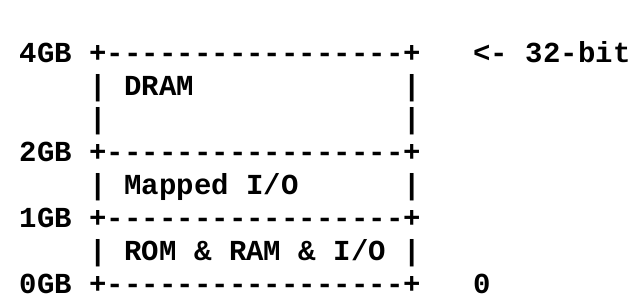
\includegraphics[scale=0.24]{arm-0-4}
        \caption{Découpage $0-4Go$}
        \label{fig:arm-0-4}
      \end{subfigure}
      \begin{subfigure}[b]{0.37\textwidth}
        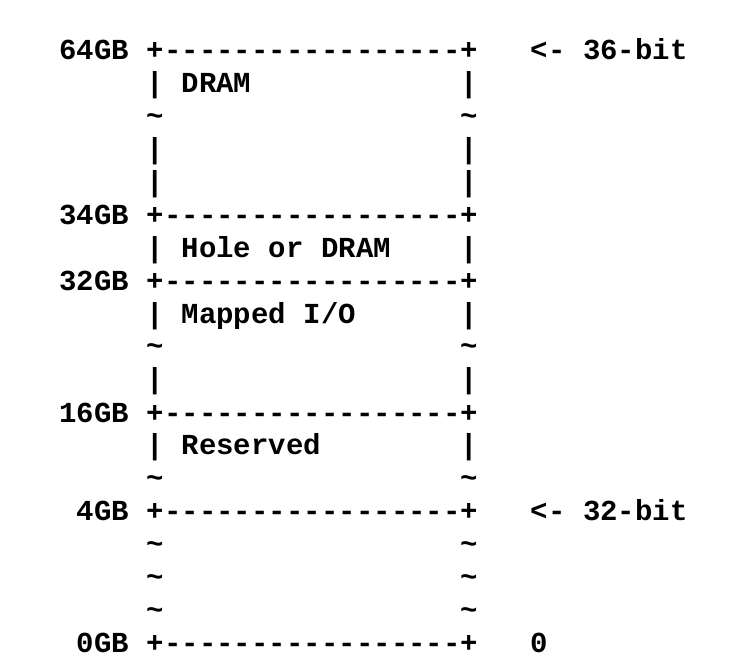
\includegraphics[scale=0.24]{arm-4-64}
        \caption{Découpage $4-64Go$}
        \label{fig:arm-4-64}
      \end{subfigure}
      \begin{subfigure}[b]{0.23\textwidth}
        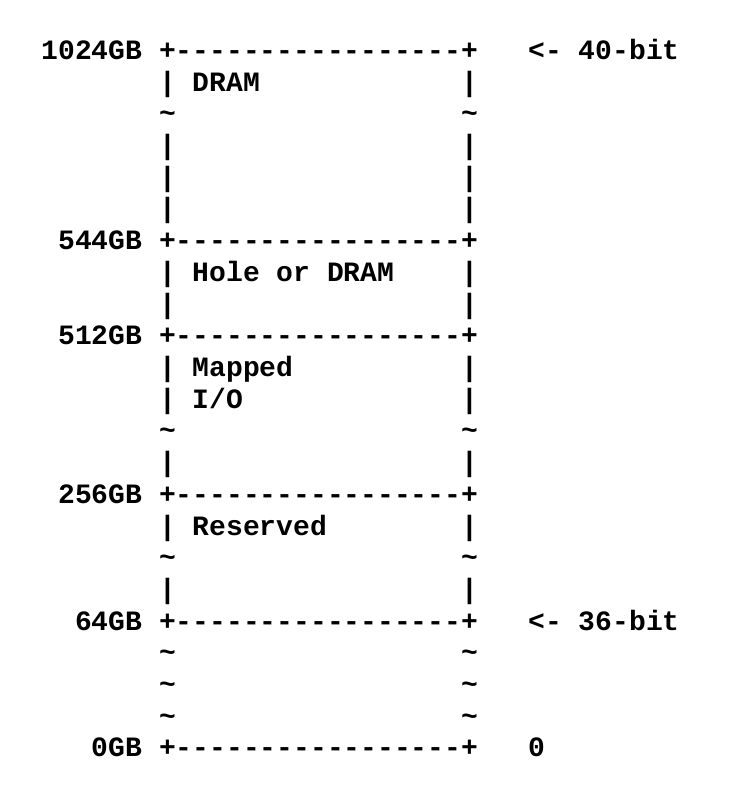
\includegraphics[scale=0.24]{arm-64-1024}
        \caption{Découpage $64-1024Go$}
        \label{fig:arm-64-1024}
      \end{subfigure}
      \caption{Découpage de l'espace mémoire sur un processeur ARMv7 avec le
        mécanisme LPAE. Source:~\citet{arm2012principles}}
      \label{fig:arm-0-1024}
    \end{figure}

    Ces derniers sont optionnels et peuvent être alloués pour des données. On
    obtient le schéma suivant:

    \begin{itemize}
      \item 512Go de données (extensible à 544Go)
      \item 273Go pour les entrées/sorties
      \item 204Go de réservés
      \item 1Go (le premier) pour la ROM, la RAM et les périphériques
        adressables
    \end{itemize}

    \todo{Pourquoi ces 204Go de réservés ?}

    Les processeurs ARM étant des processeurs RISC 32 bits, ils remplissent
    parfaitement les pré-requis nécessaires de l'architecture TSAR. De plus, ils
    sont concus de manière à avoir une (très) faible consommation électrique, ce
    qui est idéal dans notre cas. Néanmoins, l'extension LPAE

    \begin{paragraph}{Remarque:}
      L'extension LPAE supporte le mode \textit{Hypervisor} des processeurs ARM
      permettant de gérer la para-virtualisation avec des outils comme
      Xen~\cite{barham2003xen}. Bien qu'en dehors du cadre de ce stage, c'est
      une caractéristique très intéressante pour le projet
      TSUNAMY~\cite{tsunamy2013web} dans lequel l'équipe ALSOC est engagée.
    \end{paragraph}


    \subsection{Les noyaux monolithiques classiques (UNIX et NT)}

      Les noyaux monolithiques ont expoité cette avancée matérielle en
      supportant de manière logiciel le mode PAE. Pourtant, il existe des
      contraintes très fortes lorsque l'on utilise ce mode d'adressage. Dans un
      premier temps, on ne supporte que 64Go de RAM. Bien qu'énorme en 1998,
      cette valeur nous parait aujourd'hui insignifiante compte tenu de la
      puissance des machines de calcul.  Dans un second temps, cette
      amélioration apporte un problème logiciel qui reste non résolu à ce
      jour.\newline

      La mémoire est découpée de manière abstraite en pages. Ces pages peuvent
      être de grande taille (2Mo ou 4Mo selon les systèmes), ou de petite taille
      (4Ko). Pour adresser la mémoire, le noyau doit construire cette
      abstraction via les descripteurs de pages, puis toutes les opérations en
      mémoire physique passeront par ces descripteurs. Pour connaitre en
      permanence l'état global de la mémoire ou l'état d'une page en
      particulier, le noyau doit décrire entièrement l'espace
      adressable~\citep{cranor1999uvm, gorman2004understanding,
        russinovich2012windows, dillon2000design, steldt2009memory,
        steldtXXXXopenbsd}.

      Cette opération est effectuée au boot de la machine. Lorsque l’on dispose
      d’une grosse quantité de mémoire, la taille de ces descripteurs est
      énorme. À titre d’exemple, ALMOS a besoin de 14Go pour décrire les 1To de
      mémoire offerts par TSAR. Cette valeur, bien qu’élevée, est largement
      supérieure dans les noyaux Linux et *BSD, car les structures représentant
      les pages dans ces noyaux sont plus volumineuses en mémoire que celle
      d’ALMOS. Sous Linux, un descripteur de pages fait 4Ko. Pour décrire 1Go de
      mémoire, Linux a donc besoin de 11Mo\footnote{$0,044*1.10^6/4 = 11.10^3Ko
        = 11Mo$} de structure de données représentant ces pages. Si l'on
      augmente à 16Go, Linux a maintenant besoin de 176Mo pour décrire la
      mémoire. En sachant que le noyau ne s'accorde que 1Go de mémoire, et qu'il
      a besoin de ce giga-octet pour de multiple opérations, on ne peut pousser
      trop loin l'utilisation de la technologie PAE sans risquer de prendre trop
      de place en mémoire noyau et de voir des chutes de performances très
      significatives dues au mécanisme de \texttt{swap}.\\

      Le problème à résoudre est donc le suivant : comment stocker ces 14Go de
      données lorsque l’on a que 1Go d’espace virtuel ?  Actuellement, il existe
      deux réponses, toutes les deux complémentaires: \benumline \item on ne
      peut pas et \item il faut acheter une machine 64
      bits~\citep{gorman2004understanding} \eenumline. Ainsi, malgré les
      avancées matérielles, les systèmes d'exploitation n'ont pas pu explorer
      cette voie à 100\%.


  \section{Partage et maintient de cohérence de structures noyaux}
  \label{sec:consistency}
  
    %% \subsection{Hare}

    %% \subsection{Barrelfish}

    %%   passage de message

    %% \subsection{DragonFly BSD}

    %%   multi-noyau, passage de message, HAMMER
